Las características espectrales describen la representación de las señales de sonido en el dominio de las frecuencias.

Una trama $x[n]$, de longitud $N$, tiene una representación en el dominio de las frecuencias, o \textit{espectro}, que puede ser obtenida mediante la aplicación de la \textbf{transformada discreta de Fourier} (DFT por sus siglas en inglés):

\begin{equation}
    \label{eq:DFT}
    X[f] = \sum_{n=0}^{N-1}{x[n]e^{\frac{-i2\pi fn}{N}}}
\end{equation}

El espectro $X[f]$ puede ser transformado de vuelta al dominio del tiempo aplicando la \textbf{transformada discreta inversa de Fourier} (IDFT):

\begin{equation}
    \label{eq:IDFT}
    x[n] = \frac{1}{N}\sum_{f=0}^{N-1}{X[f]e^{\frac{i2\pi fn}{N}}}
\end{equation}

Al ser $x[n]$ un vector de valores reales, se puede aplicar una propiedad de la DFT que plantea que el vector $X[f]$ es por tanto conjugado simétrico, por lo que suelen considerarse solamente los últimos $\lceil (N+1)/2 \rceil$ valores de este.

La posición $k$-ésima del vector $X[k]$ contiene la amplitud correspondiente a la frecuencia $k\cdot(F_s/N)$ en la señal.

Puede definirse $X[f,t]$ como la matriz compuesta por las DFTs correspondientes a cada una de las tramas de una señal, donde el valor en la posición $\left<f, t\right>$ corresponde a la amplitud de la frecuencia $f$ en la trama $t$.
A partir de esta matriz se construye el espectrograma de la señal.

Algunas de las características más simples que pueden obtenerse directamente a partir de la DFT son las siguientes:

\begin{itemize}
    \label{itemize:basic-spectral-features}
    \item \textbf{Frecuencia pico} (\textit{Peak Frequency}): Es la frecuencia que presenta mayor magnitud en el espectro de la señal.
    \item \textbf{Amplitud pico} (\textit{Peak Amplitude}): Amplitud correspondiente a la frecuencia pico.
    \item \textbf{Frecuencias mínima y máxima} (\textbf{Min-Max Frequencies}): Menor y mayor frecuencias respectivamente, cuyas amplitudes se encuentran por encima de un valor prefijado (por ejemplo, -20 dB~\footnote{El decibelio (dB) es una unidad de medida que permite comparar relativamente dos valores siguiendo una escala logarítmica.
    La relación entre las amplitudes $A_1$ y $A_2$ está dada por la expresión $dB = 10\log(A_1/A_2)$.} respecto a la amplitud pico).
    \item \textbf{Bandwidth}: Diferencia entre las frecuencias máxima y mínima.
    \item \textbf{Cuartiles}: Caracteriza la distribución de energía en torno al espectro.
    Está compuesta por tres componentes, cada una correspondiente a la frecuencia por debajo de la que se sitúa el 25\%, el 50\% y el 75\% de la energía total del espectro respectivamente.
\end{itemize}

\subsection{Spectral Shape}\label{subsec:spectralShape}

Las características de este grupo describen la estructura del espectro de la señal;
para ello se basan en criterios estadísticos como los \textit{momentos centrales}.
A continuación se presentan tres de estas características.

\subsubsection{Spectral Centroid}\label{subsubsec:spectralCentroid}

El \textit{spectral centroid} (SC)~\cite{Fagerlund07,Kim05,Lasseck14,Manjunath02,Peters04} constituye el centro de masas del espectro de frecuencias de una trama, y permite describir la señal en términos del tipo de frecuencias predominantes (altas o bajas) en cada trama.
Puede computarse mediante la siguiente expresión:

\begin{equation}
    \label{eq:SC}
    SC = \frac{\sum_{k=0}^{K-1}{f(k)|X[k]|}}{\sum_{k=0}^{K-1}{|X[k]|}}
\end{equation}

\noindent
donde $K$ es la longitud del vector correspondiente a la DFT de la trama, y $f(k)$ la frecuencia asociada a la posición $k$-ésima de este.

\subsubsection{Spectral Spread}

También conocido como \textit{instantaneous bandwith} o \textit{spectral width}, el \textit{spectral spread} (SS)~\cite{Fagerlund07,Kim05,Manjunath02,Peters04} de una señal refleja la dispersión del espectro de frecuencias en torno a su centroide.

Puede calcularse aplicando la siguiente expresión en cada trama:

\begin{equation}
    \label{eq:SS}
    SS = \sqrt{\frac{\sum_{k=0}^{K-1}{\left[ \log_{2}{(f(k))-SC} \right]^2 |X[k]|}}{\sum_{k=0}^{K-1}{|X[k]|}}}
\end{equation}

\noindent
donde $X[k]$ es la DFT de la trama, y tiene cardinalidad $K$.

Valores bajos (característicos de sonidos armónicos) del SS expresan una concentración de las amplitudes alrededor de la frecuencia centroide;
los valores altos (propios de ruidos), en cambio, muestran una dispersión de las amplitudes en un rango de frecuencias mayor.

\subsubsection{Spectral Roll-off}\label{subsubsec:spectrallRollOff}

El \textit{spectral roll-off} (SRO)~\cite{Fagerlund07,Peters04} se define como la frecuencia bajo la cual se encuentra un porcentaje específico (usualmente entre el 85\% y el 99\%) de la energía espectral total.

\begin{figure}[!h]
    \centering
    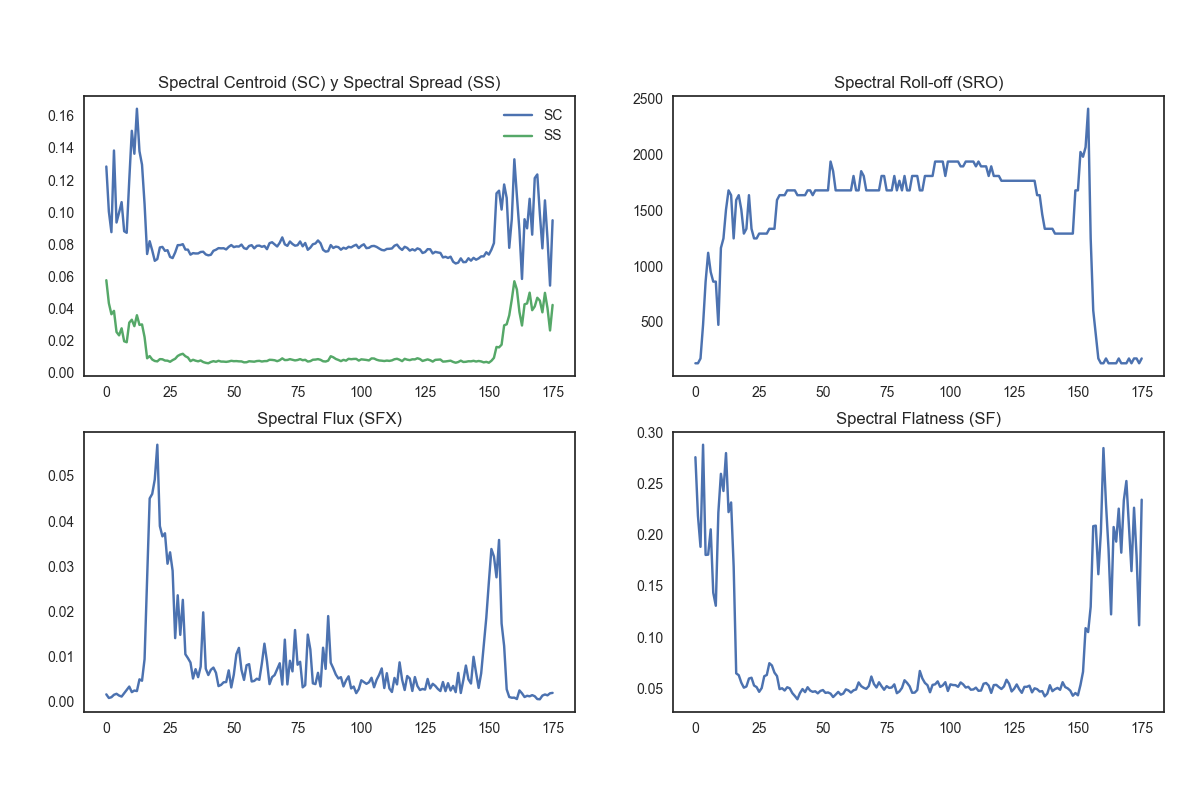
\includegraphics[width=\textwidth]{spectral-features.png}
    \caption{Características espectrales básicas de la señal de audio representada en la figura~\ref{img:oscillogram}.}
    \label{img:basic-spectral-descriptors}
\end{figure}

\subsection{Spectral Flux}\label{subsec:spectralFlux}

Caracteriza la variación dinámica de la información espectral.
El \textit{spectral flux} (SFX)~\cite{Fagerlund07,Lasseck14,Zamanian17} se calcula como la norma de la diferencia entre los espectros de dos tramas consecutivas.
El coeficiente correspondiente a la trama $t$ ($t\geq 1$) puede calcularse entonces aplicando:

\begin{equation}
    \label{eq:SFX}
    SFX_t = ||\hat{X}_t -\hat{X}_{t-1}||
\end{equation}

\noindent
donde $\hat{X}_t$ es la transformada discreta de Fourier de la trama $t$-ésima de la señal.

\subsection{Spectral Flatness}\label{subsec:spectralFlatness}

El \textit{spectral flatness} (SF)~\cite{Fagerlund07,Peters04,Zamanian17} o \textit{entropía} de una señal refleja su similitud a una señal compuesta por ruido, caso en que su valor se aproxima a 1;
mientras que si se trata de una señal armónica, el valor será próximo a 0.

El SF se calcula como la razón entre las medias geométrica y aritmética de las amplitudes presentes en la DFT de la trama, es decir, mediante la expresión:

\begin{equation}
    \label{eq:SF}
    SF = \frac{\prod_{k=0}^{K-1}{|X[k]|}^{\frac{1}{K}}}{\frac{1}{K}\sum_{k=0}^{K-1}{|X[k]|}}
\end{equation}

\noindent
donde $X[k]$ es la DFT de la trama, de cardinalidad $K$.
